\documentclass{article}
\usepackage[T1]{fontenc}
\usepackage[utf8]{inputenc}
\usepackage{lmodern}
\usepackage[T1]{fontenc}
\usepackage[utf8]{inputenc}
\usepackage{lmodern}
\usepackage[T1]{fontenc}
\usepackage[utf8]{inputenc}
\usepackage{lmodern}
\usepackage[tmargin=1cm,lmargin=1cm]{geometry}
\usepackage{tikz}
\usepackage{pgfplots}
\pgfplotsset{compat=newest}
\usepackage{pgfplots}


\begin{document}
\section{Series: h}
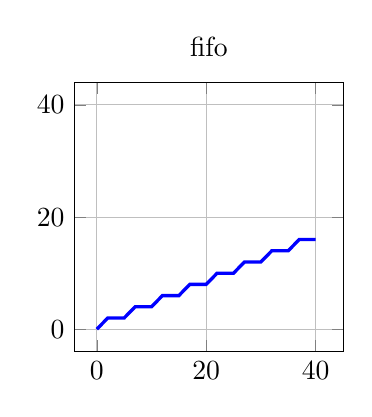
\begin{tikzpicture}
\begin{axis}[title=fifo, height=5cm, width=5cm, grid=major, xmin=({-}4.1000000000000005), xmax=(45.1), ymin=({-}4.0), ymax=(44.0)]
\addplot[very thick,color=blue] coordinates {
(0,0)
(1,1)
(2,2)
(3,2)
(4,2)
(5,2)
(6,3)
(7,4)
(8,4)
(9,4)
(10,4)
(11,5)
(12,6)
(13,6)
(14,6)
(15,6)
(16,7)
(17,8)
(18,8)
(19,8)
(20,8)
(21,9)
(22,10)
(23,10)
(24,10)
(25,10)
(26,11)
(27,12)
(28,12)
(29,12)
(30,12)
(31,13)
(32,14)
(33,14)
(34,14)
(35,14)
(36,15)
(37,16)
(38,16)
(39,16)
(40,16)
};


\end{axis}
\end{tikzpicture}
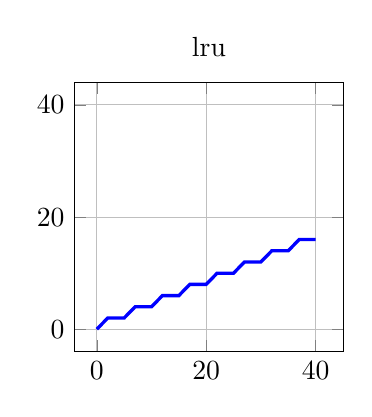
\begin{tikzpicture}
\begin{axis}[title=lru, height=5cm, width=5cm, grid=major, xmin=({-}4.1000000000000005), xmax=(45.1), ymin=({-}4.0), ymax=(44.0)]
\addplot[very thick,color=blue] coordinates {
(0,0)
(1,1)
(2,2)
(3,2)
(4,2)
(5,2)
(6,3)
(7,4)
(8,4)
(9,4)
(10,4)
(11,5)
(12,6)
(13,6)
(14,6)
(15,6)
(16,7)
(17,8)
(18,8)
(19,8)
(20,8)
(21,9)
(22,10)
(23,10)
(24,10)
(25,10)
(26,11)
(27,12)
(28,12)
(29,12)
(30,12)
(31,13)
(32,14)
(33,14)
(34,14)
(35,14)
(36,15)
(37,16)
(38,16)
(39,16)
(40,16)
};


\end{axis}
\end{tikzpicture}
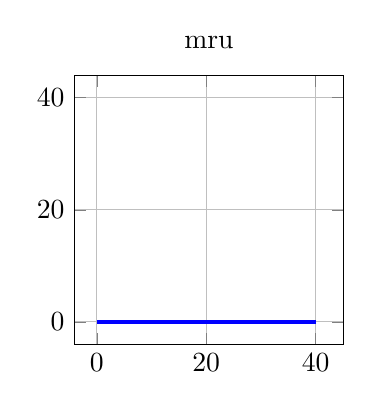
\begin{tikzpicture}
\begin{axis}[title=mru, height=5cm, width=5cm, grid=major, xmin=({-}4.1000000000000005), xmax=(45.1), ymin=({-}4.0), ymax=(44.0)]
\addplot[very thick,color=blue] coordinates {
(0,0)
(1,0)
(2,0)
(3,0)
(4,0)
(5,0)
(6,0)
(7,0)
(8,0)
(9,0)
(10,0)
(11,0)
(12,0)
(13,0)
(14,0)
(15,0)
(16,0)
(17,0)
(18,0)
(19,0)
(20,0)
(21,0)
(22,0)
(23,0)
(24,0)
(25,0)
(26,0)
(27,0)
(28,0)
(29,0)
(30,0)
(31,0)
(32,0)
(33,0)
(34,0)
(35,0)
(36,0)
(37,0)
(38,0)
(39,0)
(40,0)
};


\end{axis}
\end{tikzpicture}
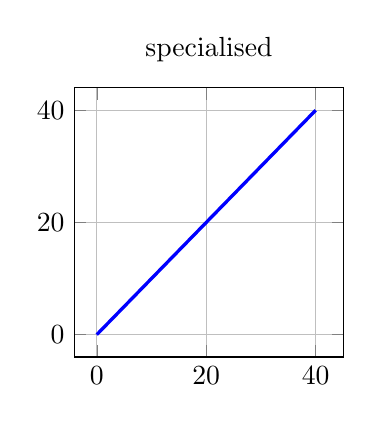
\begin{tikzpicture}
\begin{axis}[title=specialised, height=5cm, width=5cm, grid=major, xmin=({-}4.1000000000000005), xmax=(45.1), ymin=({-}4.0), ymax=(44.0)]
\addplot[very thick,color=blue] coordinates {
(0,0)
(1,1)
(2,2)
(3,3)
(4,4)
(5,5)
(6,6)
(7,7)
(8,8)
(9,9)
(10,10)
(11,11)
(12,12)
(13,13)
(14,14)
(15,15)
(16,16)
(17,17)
(18,18)
(19,19)
(20,20)
(21,21)
(22,22)
(23,23)
(24,24)
(25,25)
(26,26)
(27,27)
(28,28)
(29,29)
(30,30)
(31,31)
(32,32)
(33,33)
(34,34)
(35,35)
(36,36)
(37,37)
(38,38)
(39,39)
(40,40)
};


\end{axis}
\end{tikzpicture}


\section{Series: math.log10(h / h + ncm)}
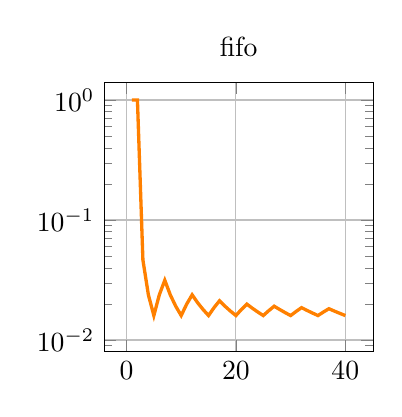
\begin{tikzpicture}
\begin{axis}[ymode=log, title=fifo, height=5cm, width=5cm, grid=major, xmin=({-}4.1000000000000005), xmax=(45.1), ymin=(0.008), ymax=(1.4)]
\addplot[very thick,color=orange] coordinates {
(1,1.0)
(2,1.0)
(3,0.046511627906976744)
(4,0.023809523809523808)
(5,0.016)
(6,0.023809523809523808)
(7,0.031496062992125984)
(8,0.023809523809523808)
(9,0.019138755980861243)
(10,0.016)
(11,0.0199203187250996)
(12,0.023809523809523808)
(13,0.020477815699658702)
(14,0.017964071856287425)
(15,0.016)
(16,0.018617021276595744)
(17,0.021220159151193633)
(18,0.019138755980861243)
(19,0.017429193899782137)
(20,0.016)
(21,0.017964071856287425)
(22,0.0199203187250996)
(23,0.01841620626151013)
(24,0.017123287671232876)
(25,0.016)
(26,0.01757188498402556)
(27,0.019138755980861243)
(28,0.017964071856287425)
(29,0.01692524682651622)
(30,0.016)
(31,0.017310252996005325)
(32,0.018617021276595744)
(33,0.017654476670870115)
(34,0.016786570743405275)
(35,0.016)
(36,0.017123287671232876)
(37,0.018244013683010263)
(38,0.017429193899782137)
(39,0.016684045881126174)
(40,0.016)
};


\end{axis}
\end{tikzpicture}
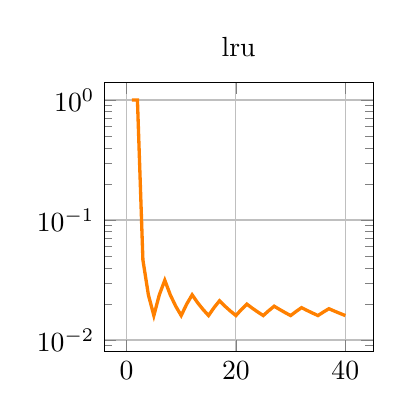
\begin{tikzpicture}
\begin{axis}[ymode=log, title=lru, height=5cm, width=5cm, grid=major, xmin=({-}4.1000000000000005), xmax=(45.1), ymin=(0.008), ymax=(1.4)]
\addplot[very thick,color=orange] coordinates {
(1,1.0)
(2,1.0)
(3,0.046511627906976744)
(4,0.023809523809523808)
(5,0.016)
(6,0.023809523809523808)
(7,0.031496062992125984)
(8,0.023809523809523808)
(9,0.019138755980861243)
(10,0.016)
(11,0.0199203187250996)
(12,0.023809523809523808)
(13,0.020477815699658702)
(14,0.017964071856287425)
(15,0.016)
(16,0.018617021276595744)
(17,0.021220159151193633)
(18,0.019138755980861243)
(19,0.017429193899782137)
(20,0.016)
(21,0.017964071856287425)
(22,0.0199203187250996)
(23,0.01841620626151013)
(24,0.017123287671232876)
(25,0.016)
(26,0.01757188498402556)
(27,0.019138755980861243)
(28,0.017964071856287425)
(29,0.01692524682651622)
(30,0.016)
(31,0.017310252996005325)
(32,0.018617021276595744)
(33,0.017654476670870115)
(34,0.016786570743405275)
(35,0.016)
(36,0.017123287671232876)
(37,0.018244013683010263)
(38,0.017429193899782137)
(39,0.016684045881126174)
(40,0.016)
};


\end{axis}
\end{tikzpicture}
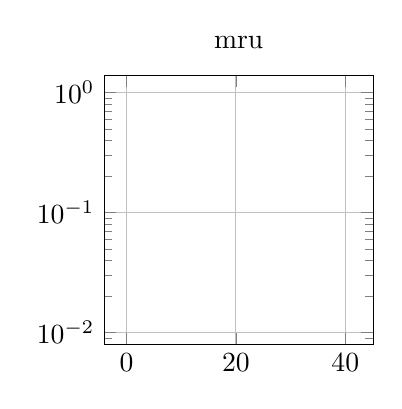
\begin{tikzpicture}
\begin{axis}[ymode=log, title=mru, height=5cm, width=5cm, grid=major, xmin=({-}4.1000000000000005), xmax=(45.1), ymin=(0.008), ymax=(1.4)]
\addplot[very thick,color=orange] coordinates {
};


\end{axis}
\end{tikzpicture}
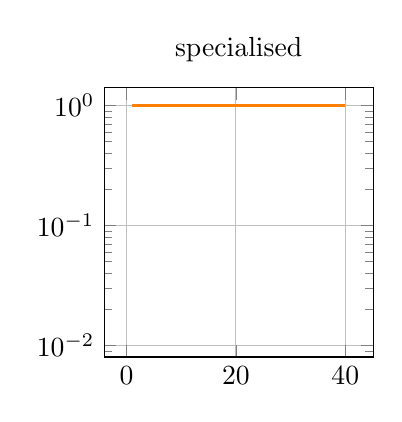
\begin{tikzpicture}
\begin{axis}[ymode=log, title=specialised, height=5cm, width=5cm, grid=major, xmin=({-}4.1000000000000005), xmax=(45.1), ymin=(0.008), ymax=(1.4)]
\addplot[very thick,color=orange] coordinates {
(1,1.0)
(2,1.0)
(3,1.0)
(4,1.0)
(5,1.0)
(6,1.0)
(7,1.0)
(8,1.0)
(9,1.0)
(10,1.0)
(11,1.0)
(12,1.0)
(13,1.0)
(14,1.0)
(15,1.0)
(16,1.0)
(17,1.0)
(18,1.0)
(19,1.0)
(20,1.0)
(21,1.0)
(22,1.0)
(23,1.0)
(24,1.0)
(25,1.0)
(26,1.0)
(27,1.0)
(28,1.0)
(29,1.0)
(30,1.0)
(31,1.0)
(32,1.0)
(33,1.0)
(34,1.0)
(35,1.0)
(36,1.0)
(37,1.0)
(38,1.0)
(39,1.0)
(40,1.0)
};


\end{axis}
\end{tikzpicture}


\end{document}